\section{Scalogram interpretation}
\label{sec:scalogram}
The data contains the time series of pixel intensities for each of the 28 ROIs for each recording of a subject, which the CWT is computed for after the signal has been corrected.  
A scalogram showing the time-frequency content of the signal is given as output of the CWT. Frequencies of higher magnitude will show up with brighter colors, which can also be seen on the magnitude colorbar for comparison of the magnitude with related values.
The frequency illustrated by the scalograms lies between 2.7370 Hz and 0.0031 Hz. This means, according to the literature, that bands of cardiac, respiratory, endothelial, myogenic and neurogenic is represented in the wavelet frequency span for the time-frequency analysis. \cite{geyer2004, sagaidachnyi2014}
An example of a raw uncorrected scalogram is shown \figref{fig:scalogram_uncorr} representing the CWT for ROI 8 from subject 3.

\begin{figure}[H]
	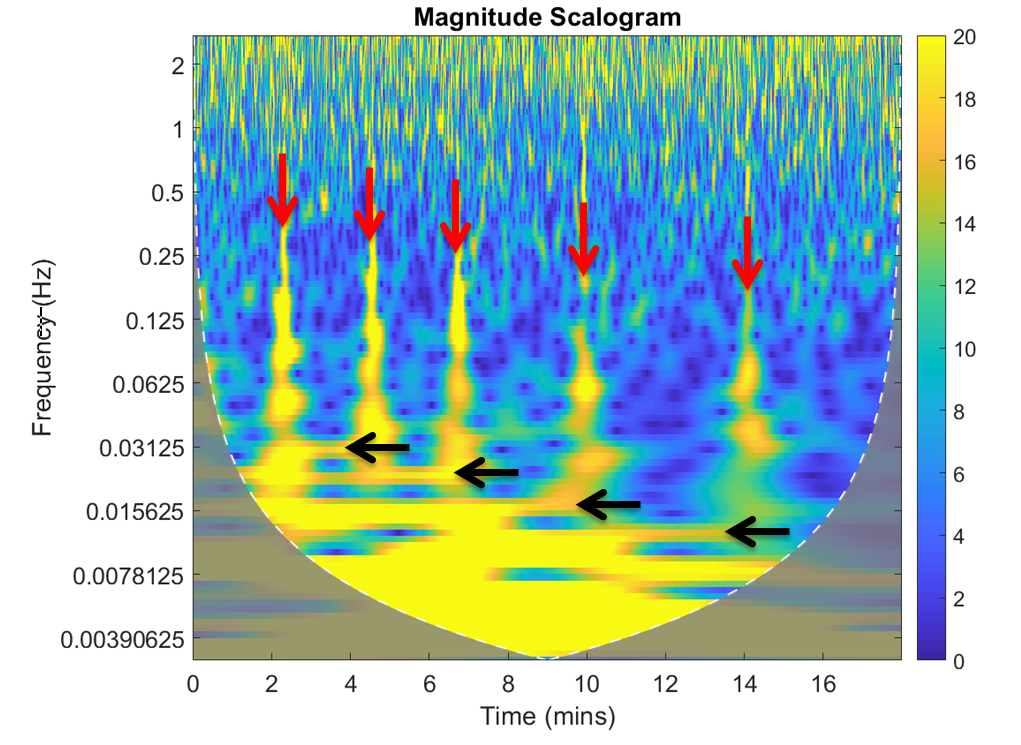
\includegraphics[width=0.7\textwidth]{figures/uncuffed_sub3_roi8_uncorr}
	\caption{Scalogram from the raw data from ROI 8 in the uncuffed recording of subject 3. Red arrows mark high spikes. Black arrows mark drifts within the intervals.}
	\label{fig:scalogram_uncorr}
\end{figure}

Looking at the scalogram from the raw signal in \figref{fig:scalogram_uncorr} the jumps can easily be seen as bright spikes which represent the jumps in the signal. Five jumps that are indicated with the red arrows, are present in the scalogram at time points around 2.5, 4.5, 6.5, 10 and 14 minute in the trace. The jumps in the same trace shown in the time domain occur at the same time points. It is presumed that the corrected drift also is represented in the scalogram as low frequency content. Hereby different artifact components can be suspected to be included in the signal content. 

The artifact components of the raw signal can be sorted into three categories: 
\begin{itemize}
	\item Uniform white noise artifacts
    \item Drift artifacts within each interval
	\item Jumps artifacts
%	\item Generel drift in the signal
\end{itemize}

Uniform white noise artifacts is characterized by having the same magnitude in all frequencies. This artifact will therefore not affect the signal of interest, because it will have a flat power spectral density throughout the bandwidth of the frequencies. White noise is independent and evenly distributed\cite{hida2014}. 
The jumps in the signal is induced by the auto-adjustments from the thermal camera described in \ref{sec:artifacts}. The drift artifacts can be seen as higher magnitudes in the scalogram as lower frequencies than the jumps. A frequency band leading up to a spike occur with each jump indicated with black arrows in \figref{fig:scalogram_uncorr}, indicating that the drift is not uniform between intervals.
The artifact components will be disturbing the trace from the micro oscillations to get a representative CWT, because this signal can be hidden by the artifacts. The artifacts are not constant for each recording, why the correction of the signal has been implemented.

\begin{figure}[H]
	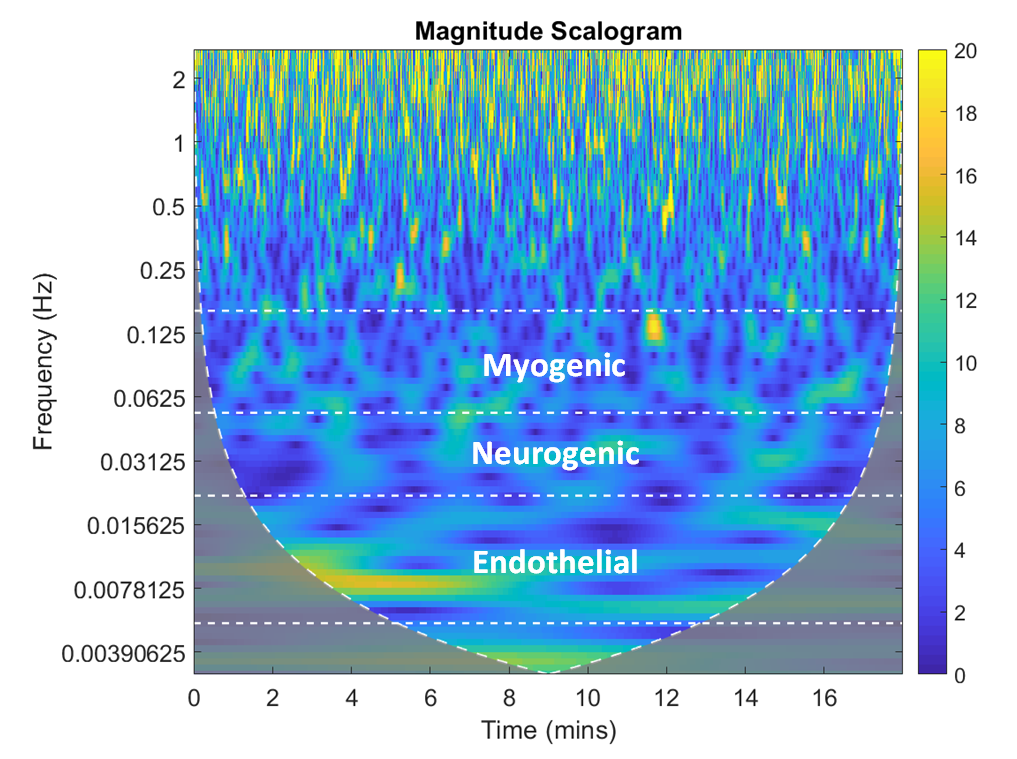
\includegraphics[width=0.7\textwidth]{figures/cwt_sub3_reg8_corr_uncuffed}
	\caption{Scalogram from the corrected data of ROI 8 in the uncuffed recording of subject 3, where a dampening of the spikes and  induced by the jumps has been achieved.}
	\label{fig:scalogram_corr}
\end{figure} 

After the correction of the signal using method 2, the energy has been reduced in the areas induced from the jumps and the drift. The scalogram is left with less energy overall as seen in \figref{fig:scalogram_corr}, also showing the range of the endothelial, neurogenic and myogenic frequency bands. %It can be discussed if the correction of the signal affects the signal of interest. 

